\documentclass[a4paper,11pt,fleqn]{article}%fleqn pour aligner les equations à gauche
\usepackage{../../Styles/Eval}


\newcommand{\chnum}{Chapitre 15 et 16}
\newcommand{\chtitle}{DS1}
\newcommand{\dtype}{DS1}

\begin{document}
\maketitle

\section{Lumière et spectres}
\begin{enumerate}
	\item Qu'est ce qu'un milieu dispersif ? (1pt)
	\item Représenter sur un schéma annoté, les phénomènes observés lorsqu'un rayon lumineux passe de l'air à l'eau. (2pt)
	\item On souhaite émettre de la lumière en chauffant un fil de cuivre. Expliquer le phénomène mis en place. (1pt)
	\item Est il possible d'émmettre une lumière verte avec cette méthode ? Justifier. (1pt)
\end{enumerate}

\section{La sonde Huygens}
Lancé en mi-octibre 1997, le couple de sondes Cassini-Huygens a parcouru durant son transit près d'une dizaine d'unités astronomiques avant d'arriver à proximité de Saturne au débit du mois de juillet 2004.\\
Au terme de leur parcours, les deux sondes se sont séparées. Si cassini est restée en orbite autour de Saturne pour effectuer le relais des transmissions avec la Terre, Huygens a réalisé son attérissage le 14 janvier 2005 sur Titan, l'un des satellites de la planète.\\
Huygens a pu fonctionner sur batterie pendant quatre heures avant de s'éteindre définitivement.\\
Le signal électromagnétique envoyé par la sonde relais Cassini devait parcourir 8,1 unités astronomiques le jour d' l'attérissage pour être reçue par la NASA sur Terre. Une unité astronomique, notée u.a., correspond à la distance Terre-Soleil. (1,0 u.a. = \SI{1,5E11}{m}).
\begin{enumerate}
	\item Déterminer une approximation de la vitesse moyenne du couple Cassini-Huygens pendant son transit jusqu'à Saturne.(2pts)
	\item Comparer cette valeur avec celui de la vitesse de la lumière.(1pt)
	\item Calculer le décalage temporel entre l'instant où le signal a été émis par la sonde et l'instant où celui-ci a été reçu sur Terre.(2pts)
\end{enumerate}



\section{L'eau de mer}
On retrouve un échantillon d'eau de mer dont on souhaite déterminer l'origine. On sait que l'indice de réfraction de l'eau salée varie selon la concentration en sel. On dispose de quelques documents ainsi que d'une expérience réalisée avec l'échantillon qui est schématisée ci-dessous.

\definecolor{waterblue}{RGB}{120,189,232}

\begin{figure}
	\begin{minipage}{.48\linewidth}
		\begin{tikzpicture}[scale=.8,transform shape]
		\fill[waterblue] (0,0) rectangle(6,-6);
		\draw (-3,0)--(6,0);
		\draw[dashed] (0,-6)--(0,6);
		\draw[line width=.08cm,orange!50!red] (-3,5.196)--(0,0);
		\draw[line width=.08cm,orange!50!red,-Stealth] (-3,5.196)to(-1.5,2.589);

		\draw[line width=.08cm,orange!50!red] (0,0)--(2.113,-6);

		\draw (3,3) node{\huge $n_{air}=1$};

		\draw (3,-3) node{\huge $n_{eausalee}$};
		
		\draw[line width=.08cm, green!40!black] (0,2) arc(90:120:2);

		\draw[line width=.08cm, green!40!black] (0,-2) arc(270:289.4:2);

		\draw[green!20!black] (0,2.5) node{\huge $i_1 = \SI{30}{\degree}$};

		\draw[green!20!black] (.5,-2.5) node{\huge $i_2$};
		\end{tikzpicture}
		\caption{Résultat de l'expérience}
	\end{minipage}\hspace{.02\linewidth}
	\begin{minipage}{.48\linewidth}
		\caption{Salinité de l'eau pour différentes mers}
		\centering
		\begin{tabular}{|c|c|}
			\hline
			\textbf{Mer considérée} & \textbf{Salinité en \unit{\gram\per\liter}}\\
			\hline
			Mer Baltique & 3 à 8\\
			\hline
			Mer Noire & 18,3 à 22,2\\
			\hline
			Océan Atlantique & 33,5 à 37,4\\
			\hline
			Océan Pacifique & 34,5 à 36,9\\
			\hline
			Océan Indien & 35,5 à 36,7\\
			\hline
			Mer Méditérranée & 38,4 à 41,2\\
			\hline
			Mer Rouge & 50,8 à 58,5\\
			\hline
			Mer Morte & 192,2 à 260 \\
			\hline
		\end{tabular}
	\end{minipage}
\end{figure}
\begin{figure}[h!]
	\centering
	\begin{tikzpicture}
		\draw[-Stealth] (0,0) to (8.5,0);
		\draw[-Stealth] (0,0) to (0,6.5);
		
		\foreach \k/\l in {0/0,1/10,2/20,3/30,4/40,5/50,6/60,7/70,8/80} {
			\draw (\k,0) -- (\k,-.1);
			\draw (\k,-.5) node{\l};
		}
		
		\foreach \k/\l in {0/1.30,1/1.35,2/1.40,3/1.45,4/1.50,5/1.55,6/1.60} {
			\draw (0,\k) -- (-.1,\k);
			\draw (-.5,\k) node{\l};
		}
		
		
		\foreach \x/\y in {0/.50,1/.98,2/1.5,3/2.3,4/2.8,5/3.5,6/4.3,7/5} {
			\draw (\x,\y) node{x};
		}
		
		\draw[domain = 0:8,color=waterblue!80!black] plot (\x, {.65*\x + 0.335});
		
		\draw (-1,6.5) node{$n_{eau salee}$};
		\draw (8.5,-1) node{concentration en sel (\unit{\gram\per\liter})};
	\end{tikzpicture}
	\caption{Valeur de l'indice de réfraction de l'eau salée en fonction de la concentration en masse de sel}
\end{figure}

\textbf{De quelle(s) région(s) du monde peu(ven)t venir cet échantillon ?} (5pts)
\end{document}

\section{Fibre optique}
Une fibre ooptique est un support de transmission utilisé par le réseau mondial Internet. Le modèle de fibre optique le plus simple, appelé fibre à saut d'indice, est constitué d'un coeur : milieu transparent d'indice $n_C$. Il est entouré d'une gaine : autre milieu transparent d'indice $n_G$.\\
Pour que la lumière se propage sans trop de pertes d'information, elle subit une série de réflexions totales à la surface de séparation entre le coeur et la gaine. Il n'y a donc pas de rayon réfracté dans la gaine.
\begin{enumerate}
	\item Exprimer l'angle de réfraction, noté $i_2$, dans le coeur de la fibre en fonction de l'angle d'incidence $i_1$ et de l'indice de réfraction $n_C$.
	\item Donner la relation entre les angles $i_2$ et $i_3$, sachant que le triangle $IJK$ est rectangle en $K$.
	\item Indiquer si le rayon lumineux qui arrive sous un angle d'incidence $i_1=\SI{32,0}{\degree}$ peut se propager dans la fibre. (représenter sur un schéma le phénomène observé)
\end{enumerate}

\begin{center}
	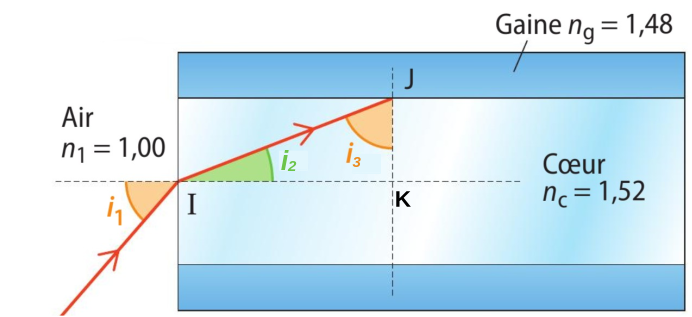
\includegraphics[width=.9\linewidth]{Resssources/2GT_DS1_Fig2.png}
\end{center}